% Adapted by M-L. Messai
\documentclass[25pt, a0paper, portrait, margin=0mm, innermargin=15mm,blockverticalspace=15mm, colspace=15mm, subcolspace=8mm]{tikzposter}

\usepackage{pgfplots}
\usepackage{booktabs}
\usepackage{multirow}
\usepackage{capt-of}
\usepackage{tcolorbox}


\input{packages}
\input{apparence}

\title{\parbox{1700pt}{Towards More Realistic Membership Inference Attacks on Large Diffusion Models}}

\author{Jan Dubiński$^1$, Antoni Kowalczuk$^{1,2}$, Stanisław Pawlak$^1$, Przemysław Rokita$^1$, Tomasz Trzciński$^{1,3,4}$,\par \hspace{0.5cm} Paweł Morawiecki$^5$}
\institute{$^1$Warsaw University of Technology, $^2$AI Society Golem, $^3$IDEAS NCBR, $^4$Tooploox, $^5$Polish Academy of Sciences}

\usetitlestyle[]{sampletitle}
\setlength{\columnseprule}{0.4pt}
\addbibresource{Biblio/Biblio.bib}

%%%%%%%%%%%%%%%%%%%%%%%%%%%%%%%%%%%%%%%%%%%%%%%%%%%%%%%%%%%
\begin{document}
\maketitle

% --- Columns
\draw[eric-lab, line width=2mm, loosely dotted] (-13,40) -- (-13,-60);
\draw[eric-lab, line width=2mm, loosely dotted] (15,40) -- (15,-25);

%------------------------------------------------------------------------------
% --------------------- Corpus of the poster ---------------------
\begin{columns}
    \column{1}
    \begin{subcolumns}
        %%%%%%%%%%%% Column 1 %%%%%%%%%%%%%
        \subcolumn{.33}

        % --------------------------------- Intro ----------

        \block{\textsc{TL;DR}}{
    \begin{itemize}{
        \item We identify the \textbf{pitfalls} of existing approaches to \textit{membership inference attacks} on large diffusion models.
        \item We provide a new \textbf{dataset} along with construction methodology.
        \item We propose a \textbf{fair} and \textbf{rigorous} evaluation protocol on the \textbf{SOTA Stable Diffusion model}.
        \item We thoroughly evaluate a set of \textit{MIAs} using our dataset and methodology.
    }\end{itemize}
}


        % --------------------------------- MIA ----------

        \block{\textsc{Membership Inference Attacks}}{
    Was this example used to train the model? \textbf{Yes} or \textbf{No}?
    \begin{center}
        % [trim={left bottom right top},clip]
        \includegraphics[width=1.05\linewidth,trim={1cm 0 0.5cm 0.5cm}]{images/figures/loss_thrs.pdf}
    \end{center}
    \textbf{Loss Threshold Attack}: $IF\ loss(sample)<threshold\ THEN\ member\ ELSE\ nonmember$.
}


        % --------------------------------- Approaches  ----------    

        \block{\textsc{Problem: lack of nonmembers set}}{
    \textit{We cannot run MIA evaluation without nonmembers}. A few approaches has been proposed:
    \begin{enumerate}{
        \item Fine-tune Stable Diffusion on a new dataset\cite{duan2023diffusion}. \textbf{Pitfall}: too trivial problem due to overfitting.
        \item Train a new model on a new dataset. \textbf{Problem}: too expensive.
        \item Create a dataset with similar properties to the original one. \textbf{Challenge}: distribution mismatch.
    }\end{enumerate}
}



        % ---------------------------------  POKEMON Teaser ----------

        \block{\textsc{Pitfall: Fine-tuning}}{
    \begin{center}
        \includegraphics[width=1.05\linewidth]{images/figures/teaser.pdf}
    \end{center}
    \small Pitfalls in the evaluation setting can lead to incorrect conclusions on the effectiveness of \textit{membership inference attacks} against large diffusion models such as Stable Diffusion.
}



        %%%%%%%%%%%%%%% Column 2 %%%%%%%%%%%%%

        \subcolumn{.33}

        % ------------------------------------ LAION-mi dataset ------------

        \block{\textsc{LAION-mi Dataset}}{
    \begin{center}
        \includegraphics[width=\linewidth]{images/figures/LAION-mi-scheme_3.pdf}
    \end{center}
    A general scheme of constructing LAION-mi dataset.
}



        % ------------------------------------ Challenges ------------

        \block{\textsc{Challenges}}{
    \begin{itemize}{
        \item Duplicates: LAION-2B EN constains ~30\% duplicates\cite{webster2023deduplication}.
        \item Distribution mismatch: LAION-2B EN and LAION-2B Multi Translated may have different distributions.
    }\end{itemize}
}


        % ------------------------------------ Deduplication plots ------------

        \block{\textsc{Deduplication}}{
    \begin{minipage}{0.5\linewidth}
        \includegraphics[width=\textwidth]{images/figures/l2-dist.pdf}
        \small Distribution of L2 distances. \newline
    \end{minipage}
    \hspace{0.05\linewidth}
    \begin{minipage}{0.5\linewidth}
        \includegraphics[width=\textwidth]{images/figures/l2-dist-duplicates.pdf}
        \small Duplicates count per 100 samples for L2 distances buckets.
    \end{minipage}
}

        % ------------------------------------ Evaluation table ------------

        \block{\textsc{Evaluation}}{
    \begin{minipage}{\linewidth}
        \begin{tabular}{c c c c c}
    \toprule
                                &                               &                        & \multicolumn{2}{c}{\textbf{TPR@FPR=1\%. $\uparrow$}}                      \\
    \textbf{Scenario}           & \textbf{Loss}                 & \textbf{Method}        & \textbf{ LAION-mi}                                   & \textbf{POKEMON}   \\

    \midrule
    \multirow{10}{*}{White-box} & \multirow{4}{*}{Model Loss}   & Baseline loss thr.     & 1.92\%$\pm$0.59                                      & 80.9\%$\pm2.27$    \\
    %  Duan stat & -\% &  -\%\\
    % Duan NN & -\% & -\%\\
    \cmidrule{3-5}

                                &                               & Reversed noising       & 2.51\%$\pm$0.73                                      & 97.3\%$\pm0.93$    \\
                                &                               & Partial denoising      & 2.31\%$\pm$0.61                                      & 94.5\%$\pm1.34$    \\
                                &                               & Reversed denoising     & 2.25\%$\pm$0.64                                      & 91.5\%$\pm1.63$    \\


    \cmidrule{2-5}

                                & \multirow{3}{*}{Latent Error} & Reversed noising       & 1.26\%$\pm$0.62                                      & 11.5\%$\pm1.84$    \\
                                &                               & Partial denoising      & 2.42\%$\pm$0.62                                      & 99.5\%$\pm0.4$   \\
                                &                               & Reversed denoising     & 2.17\%$\pm$0.64                                      & 61.1\%$\pm2.74$    \\

    \cmidrule{2-5}


                                & \multirow{3}{*}{Pixel Error}  & Reversed noising       & 1.90\%$\pm$0.51                                      & 8.36\%$\pm1.66$    \\
                                &                               & Reversed denoising     & 2.03\%$\pm$0.55                                    & 12.0\%$\pm1.97$    \\
                                &                               & Partial denoising      & 1.75\%$\pm$0.68                                      & 25.38\%$\pm2.55$ \\
    \midrule

    Grey-box                    & Latent Error                  & Generation from prompt & 0.93\%$\pm$0.41                                      & 7.15\%$\pm1.5$     \\
    \midrule
    Black-box                   & Pixel Error                   & Generation from prompt & 0.35\%$\pm$0.19                                      & 12.0\%$\pm1.9$     \\
    \bottomrule
\end{tabular}
    \end{minipage}
}

        \block{}{
            \vspace*{-4cm}
            \printbibliography
        }

        %%%%%%%%%%%%%%%%%%%%%%%% Column 3 %%%%%%%%%%%%%%%%%%%%%%%%%   

        \subcolumn{.33}

        % ------------------------------------ Distribution check ------------

        \block{\textsc{Distribution Mismatch}}{
    We assess the mismatch using the following metrics:
    \begin{itemize}{
        \item Visual inspection of the PCA projection of the dataset.
        \item FID score between the subsets.
        \item Classifier-based evaluation.
    }\end{itemize}
}


        % ------------------------------------ PCA plots ------------

        \block{\textsc{Sanitization: PCA Projection}}{
    \begin{minipage}{0.5\linewidth}
        \includegraphics[width=\textwidth]{images/figures/single-prompts_before_sanitization.png}
        \small Prompts before sanitization. \newline
    \end{minipage}
    \hspace{0.05\linewidth}
    \begin{minipage}{0.5\linewidth}
        \includegraphics[width=\textwidth]{images/figures/single-prompts_iteration_3.png}
        \small Prompts after sanitization.
    \end{minipage}
}

        % ------------------------------------ FID table ------------

        \block{\textsc{Sanitization: FID}}{
    \begin{minipage}{\linewidth}
        \begin{tabular}{@{}lcc@{}}
    \toprule
                                 & \multicolumn{2}{c}{FID}                 \\
    Data subset                  & text                    & images        \\
    \midrule
    Members internal - random    & 9.84                    & 7.00          \\
    Members internal - sanitized & 9.77                    & 7.06          \\
    Nonmembers internal          & 9.73                    & 7.01          \\
    \midrule
    Comparative - random         & 66.43                   & 13.90         \\
    Comparative - sanitized      & \textbf{13.54}          & \textbf{8.87} \\
    \bottomrule
\end{tabular}
    \end{minipage}
}


        % ------------------------------------ LAION-mi pics ------------

        \block{\textsc{LAION-mi Samples}}{
    \begin{minipage}{0.5\linewidth}
        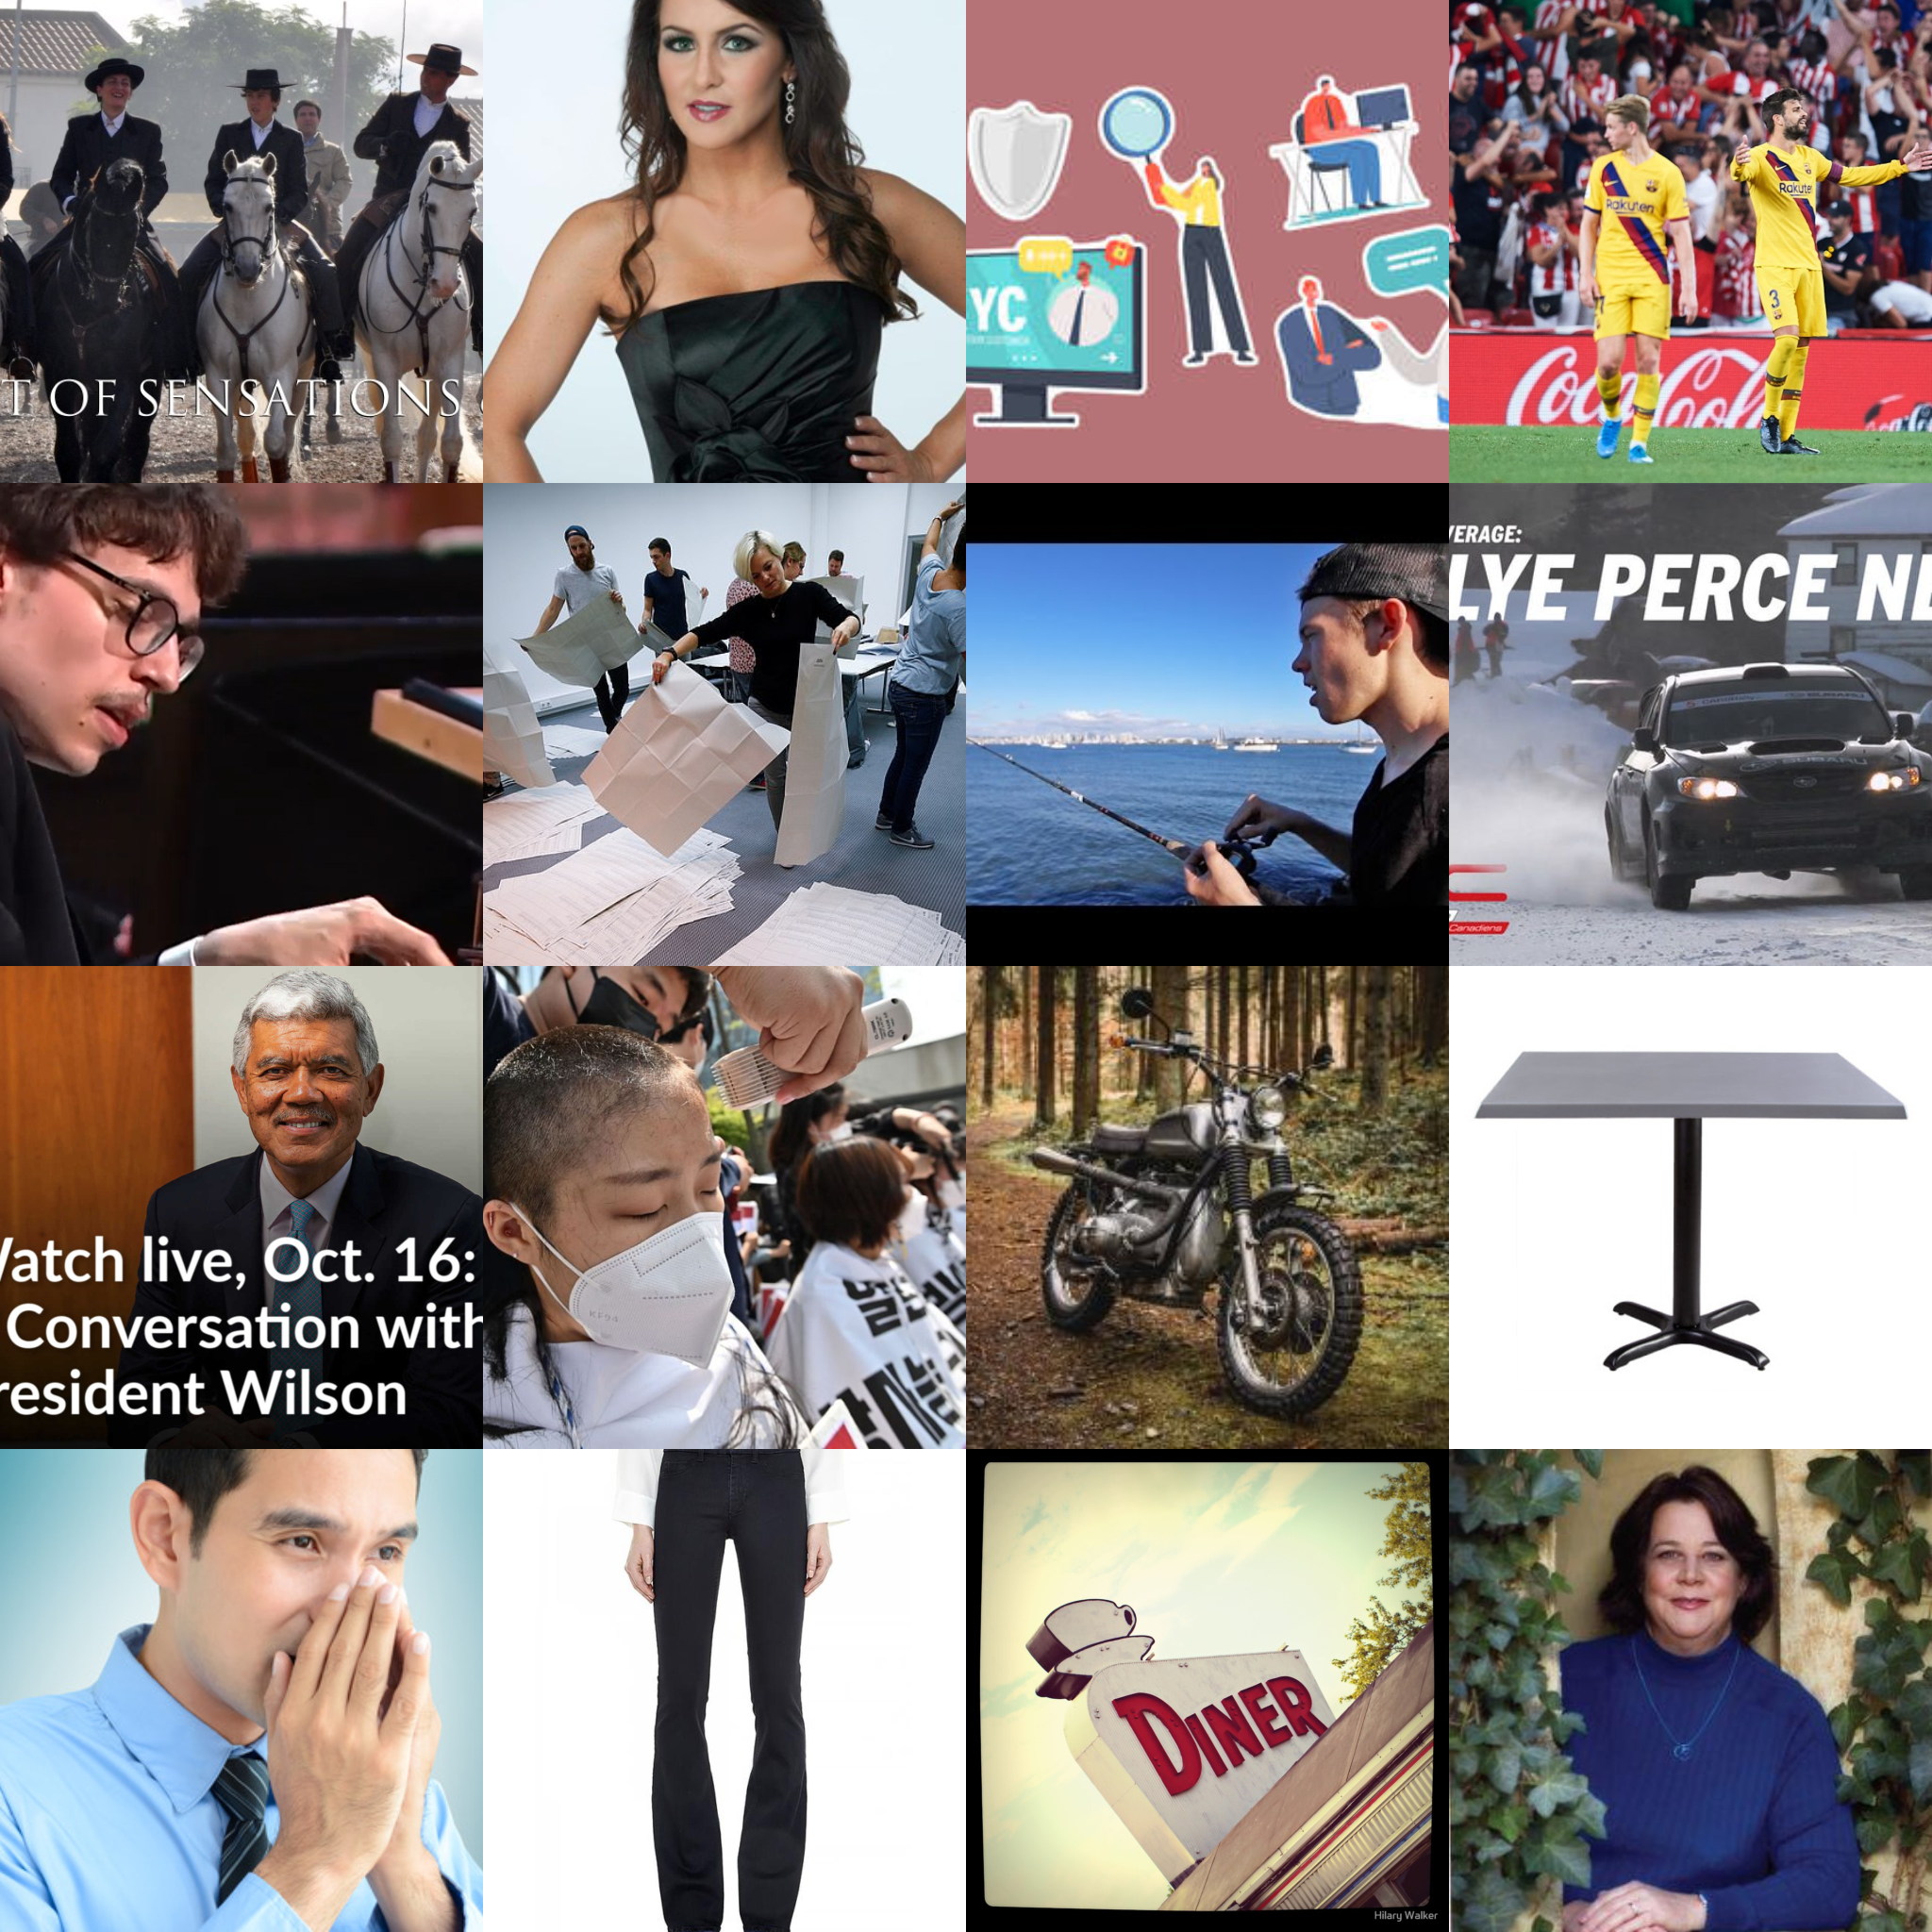
\includegraphics[width=\textwidth]{images/figures/laion_mi_vis_m.png}
        \small Sample 16 members. \newline
    \end{minipage}
    \hspace{0.05\linewidth}
    \begin{minipage}{0.5\linewidth}
        
\includegraphics[width=\textwidth]{images/figures/laion_mi_vis_nm.png}
        \small Sample 16 nonmembers.
    \end{minipage}
}

        % ------------------------------------ QR code to paper ------------

        \hspace*{8cm}
\block{}{
    \begin{tcolorbox}[sharp corners, colframe=eric-lab, colback=white, width=14cm, boxrule=5pt]
        \center\LARGE\textsc{\textcolor{eric-lab}{\textbf{Paper}}} \\
        \vspace*{1cm}
        \includegraphics[width=\textwidth]{images/figures/qr_paper.png}
    \end{tcolorbox}
}

    \end{subcolumns}


    % ---------------------------------  References ----------

\end{columns}

% ----------------- Footer -------------
\node [above right, text=white,outer sep=45pt,minimum width=\paperwidth, align=center, draw, fill=titledarkcolor, color=Orange] at (-51.6,-61) { \textcolor{white}{\normalsize Contact: antonikowalcz@gmail.com}};

\end{document}
